\begin{figure}[bth!]
  \begin{center}
    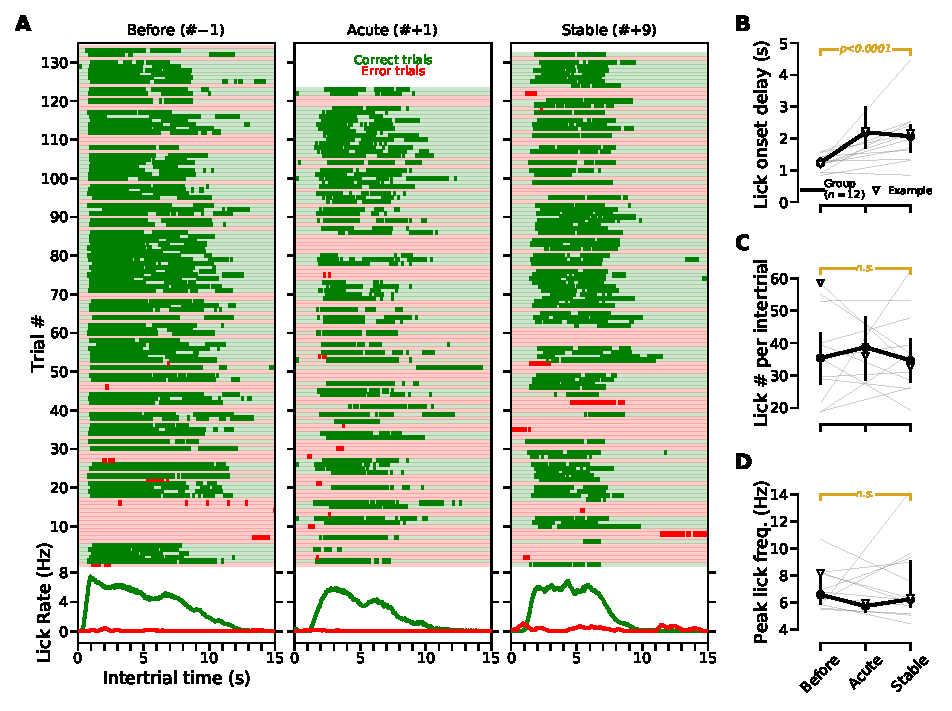
\includegraphics[width=1\linewidth]{ch-lesion/figures/Lick.pdf}
    \caption
    {\textbf{Licking behavior after dS lesion.}
	\textbf{(A)} Trial-by-trial licking patterns (top) and averaged lick rate aligned to intertrial onset for a single animal in 3 sessions (1 just before and 2 after lesion). 
	\textbf{(B-D)} Effect of dS lesion on lick onset delay (B), number of licks per intertrial (C) and peak lick frequency (D)
	}
	\label{fig:lesion:lick}
  \end{center}
\end{figure}